%================================================
% Section 1.2: Formulas for the Green's Functions
%================================================
\documentclass[../dissertation.tex]{subfiles}
\def\rest{\text{rest}}

\begin{document}
\section{Green's Function Contour Shift}\label{sec1:GreensFunctions}
Now that we know the integrand for $G_L^+$, $G_R^+$ has exactly two poles in 
a strip about the real line, we are now able to use
contour shifts to derive representation formulas for $G_L^+$ and $G_R^+$ which we use to study the 
mapping properties of these operators. 


To simplify our analyses, we first note that $G_L^+$ and $G_R^+$ have
the useful scaling (in $\delta$) and conjugate properties shown in 
Proposition \ref{prop1:DiaConj}.
\begin{prop}\label{prop1:DiaConj}
	The Green's Functions $G_L^+$ and $G_R^+$ satisfy the following
	identities:
	\begin{itemize}
		\item[(i)] $\ds G_\star^+(x; \lambda, \delta) 
			= G_\star^+(x/\delta; \delta\lambda, 1)$
		\item[(ii)] $\ds G_R^+(x; \lambda, \delta) = \ol{G_L^+(-x;\lambda, \delta)}$,
	\end{itemize}
	where, as mentioned in Remark \ref{rmk1:StarNotation}, we use the $\star$ in the 
	notation in $G_\star^+$ is a stand-in for either
	$L$, or $R$. That is, both $G_L^+$ and $G_R^+$ satisfy identity (i).
\end{prop}
\begin{proof}
	To prove (i), observe that 
	\[
		\zeta(\xi; \delta) 
			= \frac{\xi e^{\delta \xi}}{e^{\delta \xi} - e^{-\delta \xi}}
			= \delta^{-1} \frac{ \delta \xi e^{\delta \xi}}{e^{\delta \xi} - e^{-\delta \xi}}
			= \delta^{-1} \zeta(\delta \xi; 1).
	\]
	As such 
	\begin{align}\label{eq1:pdia}
		p(\xi; \lambda, \delta) 
			= \big( \zeta(\xi; \lambda) - \zeta(\lambda) \big) \( 1- e^{-2 \delta \xi} \)
			= \delta^{-1} p(\delta \xi; \delta \lambda, 1).
	\end{align}
	Recalling that $G_\star^+$ can be written in the form
	\[
		G_L^+(x; \lambda, \delta)
			= \frac{1}{2 \pi} \mathop{\int}_{\mathbb R - i0} 
				\frac{e^{i x \xi}}{p(\xi , \lambda ; \delta)} \, \mathrm{d} \xi,
		\qquad 
		G_R^+(x; \lambda, \delta)
			= \frac{1}{2 \pi} \mathop{\int}_{\mathbb R + i0} 
				\frac{e^{i x \xi}}{p(\xi , \lambda ; \delta)} \, \mathrm{d} \xi,
	\]
	where we use the convention that $(\dotarg \pm i0)$\label{sym:i0} implies a limit 
	involving $(\dotarg \pm i \ve)$ as $\ve \searrow 0$, equation \ref{eq1:pdia}
	implies that the Green's Functions $G_\star^+$ satisfy scaling identity (i),
	as 
	\[
		\frac{1}{2 \pi} \mathop{\int}_{\mathbb R \mp i 0} 
				\frac{ e^{i \(\frac{x}{\delta}\) (\delta\xi)}}{p(\xi, \lambda; \delta)} \, \mathrm{d}\xi	
			= \frac{1}{2 \pi} \, \delta \mathop{\int}_{\RR \mp i 0} 
				\frac{ e^{i \(\frac{x}{\delta}\) (\delta\xi)}}{p(\delta \xi, \delta \lambda; 1)} \, \mathrm{d}\xi
			= \frac{1}{2 \pi} \mathop{\int}_{\RR \mp i 0}  
				\frac{ e^{i \(\frac{x}{\delta}\) \xi}}{p(\xi, \delta \lambda; 1)} \, \mathrm{d}\xi.
	\]
	Further, the computation
	\[
		G_R^+(x; \lambda, \delta) 
			= \frac{1}{2 \pi } \mathop{\int}_{\RR+i0} 
				\frac{\ol{e^{i (-x)\xi}}}{p(\xi,  \lambda)} \, \mathrm{d}\xi
			= \frac{1}{2 \pi } \ol{\mathop{\int}_{\RR-i0} 
				\frac{e^{i (-x)\xi}}{p(\xi,  \lambda)} \, \mathrm{d}\xi}
			= \ol{G_L^+(-x; \lambda, \delta)},
	\]
	verifies identity (ii) and completes this proof.
\end{proof}

\begin{rmk}\label{rmk1:contin}
	In Chapter \ref{cptr03:xContin}, we show that $G_\star^+$ ($\star = L \text{, or } R$)
	has an analytical extension $G_\star$ to the strip 
	\[
		\mathcal S_\delta = \{ z \in \mathbb C ~:~ 0 < \im z < 2\delta \}
	\]
	with upper boundary value
	$G_\star^-$. Since the arguments in the above proof still hold when $x$ is 
	replaced with $x + iy$, ($x\in \mathbb R$ and $0< y<2\delta$), we take without
	proof that the functions $G_\star$ satisfy the corresponding identities
	\begin{itemize}
		\item[(i)] $\ds G_\star(z; \lambda, \delta) 
			= G_\star(z/\delta; \delta\lambda, 1)$
		\item[(ii)] $\ds G_R(x+iy; \lambda, \delta) = \ol{G_L(-x+iy;\lambda, \delta)}$,
	\end{itemize}
	for $z \in \mathcal S_\delta$, $x \in \mathbb R$, and $0< y < 2\delta$. 
\end{rmk}

\begin{rmk}\label{rmk1:wlog}
	Proposition \ref{prop1:DiaConj} in conjunction with Remark \ref{rmk1:contin} allows 
	us to focus our analysis on $G_L(z; \lambda, 1)$ on its boundary values
	$G_L^\mp(x; \lambda, 1)$ and deduce the corresponding results for 
	$G_L(z; \lambda, \delta)$ and $G_R(z; \lambda, \delta)$. As such, unless otherwise 
	explicitly stated, we take $\delta = 1$ throughout the remainder of this 
	dissertation and commonly suppress the $\delta$ dependence of the functions we
	analyze. For example, we will often write $G_L^+(x)$ or $G_L^+(x; \lambda)$ instead
	of $G_L^+(x; \lambda, \delta)$.
\end{rmk}

The discussion that follows is based on integrating
$e^{ix\xi} / p(\xi)$ around the contour shown in Figure \ref{fig1:GammaContour}
under the assumption that $\lambda \ne 0$.
Recalling from Section \ref{sec1:RootsOfP} that the only roots of $p$ contained 
in the strip
\[
	\mc S_1 = \big\{ \xi \in \mathbb C ~:~ -\pi \leq \im \xi \leq \pi \big\}
\]
are $\xi = 0$ and $\xi = \lambda$, integrating $e^{ix\xi} / p(\xi)$ around such a 
contour is allowed. In the case where $\lambda=0$, then the contours shown in 
Figure \ref{fig1:GammaContour} contain a single circular arc arround the pole
at $\xi = 0$. 


The function $e^{ix\xi}$ has an analytic continuation to the upper complex $\xi$ 
plane for $x > 0$ and an analytic continuation to the lower complex $\xi$ plane
when $x < 0$. So, for fixed $\ve > 0$ with $\ve < \min\{\lambda /2, \, \pi\}$, define 
the counter-clockwise oriented contours $\Gamma(R, \ve, x, \lambda)$ as shown below in 
Figure \ref{fig1:GammaContour} and 
note that the integrand of $G_L^+(x, \lambda, 1)$ is analytic along $\Gamma(R, \ve, x, \lambda)$.

\begin{figure}[H]
	\centering
	\begin{subfigure}[t]{0.49\textwidth}
		\centering
		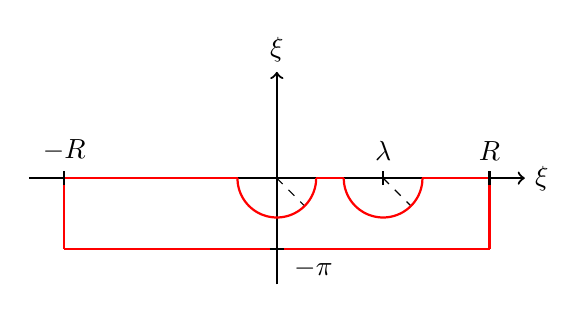
\begin{tikzpicture}[
				scale=0.9,
				cont/.style={red, smooth, thick}
			]
			\def\R{3}
			\def\lambdaam{\R/2}
			\def\ep{\lambdaam/2.7}
			\def\XaxisScale{0.5}
			\def\YaxisScale{0.5}
			\def\tickLength{0.1}
			\def\width{1.0}

			% Draw real and imaginary axes
			\draw[->, thick] ({-\XaxisScale-\R}, 0) -- ({\XaxisScale+\R}, 0)
				node[right] {$\re \xi$};
			\draw[->, thick] (0, {-\YaxisScale-\width}) -- (0, {\YaxisScale+\width})
				node[above] {$\im \xi$};

			% Draw Radii
			\path[dashed] (0, 0) edge node[pos=0.3, below] {$\ve$} 
				({\ep*cos(-45)},{\ep*sin(-45)});
			\path[dashed] ({\lambdaam}, 0) edge node[pos=0.3, below] {$\ve$} 
				({\ep*cos(-45) + \lambdaam},{\ep*sin(-45)});

			% Draw the contour
			\draw[cont, domain={-\R}:{0-\ep}, variable=\x] plot ({\x}, 0);
			\draw[cont, domain={0+\ep}:{\lambdaam-\ep}, variable=\x] plot ({\x}, 0);
			\draw[cont, domain={\lambdaam+\ep}:\R, variable=\x] plot ({\x}, 0);
			\draw[cont, domain=0:{\width}, variable=\y] plot ({-\R}, -\y);
			\draw[cont, domain=0:{\width}, variable=\y] plot ({\R}, -\y);
			\draw[cont, domain={-\R}:{\R}, variable=\x] plot ({\x}, {-\width});

			\draw[cont, domain=180:360, variable=\th]
				plot ({\ep*cos(\th)}, {\ep*sin(\th)});
			\draw[cont, domain=180:360, variable=\th]
				plot ({\ep*cos(\th)+\lambdaam}, {\ep*sin(\th)});

			% Draw ticks
			\draw[thick] ({-\R}, {-\tickLength}) -- ({-\R}, {\tickLength})
				node[above] {$-R$};
			\draw[thick] ({\R}, {-\tickLength}) -- ({\R}, {\tickLength})
				node[above] {$R$};
			\draw[thick] (\lambdaam, {-\tickLength}) -- ({\lambdaam}, {\tickLength})
				node[above] {$\lambda$};
			\draw[thick] ({-\tickLength}, {-\width}) -- ({\tickLength}, {-\width})
				node[below right] {$-\pi$};

		\end{tikzpicture}
		\caption{The contour $\Gamma(R, \ve, x ,\lambda)$ for $x < 0$}
		\label{fig1:GammaContourA}
	\end{subfigure}
	\begin{subfigure}[t]{0.49\textwidth}
		\centering
		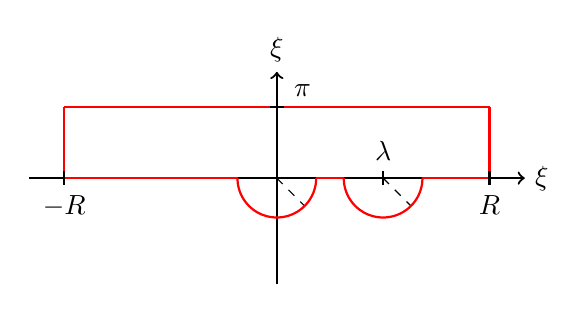
\begin{tikzpicture}[
				scale=0.9,
				cont/.style={red, smooth, thick}
			]
			\def\R{3}
			\def\lambdaam{\R/2}
			\def\ep{\lambdaam/2.7}
			\def\XaxisScale{0.5}
			\def\YaxisScale{0.5}
			\def\tickLength{0.1}
			\def\width{1.0}

			%% Draw real and imaginary axes
			\draw[->, thick] ({-\XaxisScale-\R}, 0) -- ({\XaxisScale+\R}, 0)
				node[right] {$\re \xi$};
			\draw[->, thick] (0, {-\YaxisScale-\width}) -- (0, {\YaxisScale+\width})
				node[above] {$\im \xi$};

			%% Draw Radii
			\path[dashed] (0, 0) edge node[pos=0.3, below] {$\ve$} 
				({\ep*cos(-45)},{\ep*sin(-45)});
			\path[dashed] ({\lambdaam}, 0) edge node[pos=0.3, below] {$\ve$} 
				({\ep*cos(-45) + \lambdaam},{\ep*sin(-45)});

			%% Draw the contour
			\draw[cont, domain={-\R}:{0-\ep}, variable=\x] plot ({\x}, 0);
			\draw[cont, domain={0+\ep}:{\lambdaam-\ep}, variable=\x] plot ({\x}, 0);
			\draw[cont, domain={\lambdaam+\ep}:\R, variable=\x] plot ({\x}, 0);
			\draw[cont, domain=0:{\width}, variable=\y] plot ({-\R}, \y);
			\draw[cont, domain=0:{\width}, variable=\y] plot ({\R}, \y);
			\draw[cont, domain={-\R}:{\R}, variable=\x] plot ({\x}, {\width});

			\draw[cont, domain=180:360, variable=\th]
				plot ({\ep*cos(\th)}, {\ep*sin(\th)});
			\draw[cont, domain=180:360, variable=\th]
				plot ({\ep*cos(\th)+\lambdaam}, {\ep*sin(\th)});


			%% Draw ticks
			\draw[thick] ({-\R}, {\tickLength}) -- ({-\R}, {-\tickLength})
				node[below] {$-R$};
			\draw[thick] ({\R}, {\tickLength}) -- (\R, {-\tickLength})
				node[below] {$R$};
			\draw[thick] (\lambdaam, {-\tickLength}) -- (\lambdaam, {\tickLength})
				node[above] {$\lambda$};
			\draw[thick] ({-\tickLength}, {\width}) -- ({\tickLength}, {\width})
				node[above right] {$\pi$};

		\end{tikzpicture}
		\caption{The contour $\Gamma(R, \ve, x, \lambda)$ for $x > 0$}
		\label{fig1:GammaContourB}
	\end{subfigure}
	\caption{Contours for shifting the contour of integration for 
		$G_L$ of{}f of the real line.}
	\label{fig1:GammaContour}
\end{figure}

By the reverse triangle inequality,
\begin{align*}
	|p(\xi)| \geq \Big| |\xi| - \zeta(\lambda)\left| 1 - e^{-2\xi} \right|  \Big|.
\end{align*}
Since 
\[
	\left| 1 - e^{-2 \xi} \right|^2
		= \( 1 - e^{-2 \xi} \) \( 1 - e^{-2 \ol \xi} \)
		= 1 - 2 \re e^{-2\xi} + e^{-4 \re \xi},
\]
and 
\[
	\re  e^{-2 \xi} = e^{\mp 2R} \cos(-2y)
\]
for $\xi = \pm R + i y$ ($y \in \RR$),
we find 
\begin{align*} %\label{eq:pLowerBnd}
	\lim_{R\to\infty} \big| p(\pm R + iy) \big|
		\geq \lim_{R\to\infty} \left| \sqrt{R^2 + y^2} 
			- \zeta(\lambda) \( 1 - e^{\mp2R}\cos(-2y) + e^{\mp 4R} \)^{\frac{1}{2}} \right|
		= \infty.
\end{align*}
Thus, 
\begin{align} \label{eq1:GammaSides}
	\lim_{R\to\infty} \left|\frac{e^{ix(\pm R + iy)}}{p(\pm R + iy)}\right|
		= 0,
\end{align}
which implies that the contributions of the sides of $\Gamma(R, \ve, x, \lambda)$ to the 
overall value of the integral $\mathop{\int}_\Gamma e^{ix\xi}/p(\xi)\, \mathrm{d}\xi$ goes to zero
as we take $R \to \infty$. Cauchy's theorem in conjunction with 
\eqref{eq1:GammaSides} consequently tell us that  
\begin{align} \label{eq1:Gffraw}
	G_L^+(x; \lambda) =
		\begin{cases}
			\ds \frac{1}{2\pi} \int\limits_{\mathbb R-i\pi} \frac{e^{ix\xi}}{p(\xi)} \, \mathrm{d}\xi, 
				&  x < 0 \\ ~\\
			\ds i \, \Res_{\xi = 0}\( \frac{e^{ix\xi}}{p(\xi)} \)
			+ i \, \Res_{\xi = \lambda}\( \frac{e^{ix\xi}}{p(\xi)} \)
			\frac{1}{2\pi} \mathop{\int}_{\RR+i\pi} \frac{e^{ix\xi}}{p(\xi)} \, \mathrm{d}\xi, 
				&  x > 0 
		\end{cases}
\end{align}
where
\[
	\Res_{\xi = 0}\( \frac{e^{ix\xi}}{p(\xi)} \) 
		= \frac{1 - e^{2\lambda}}{2\lambda e^{2\lambda} + 1 - e^{2\lambda}},
	\qquad \text{and} \qquad
	\Res_{\xi = \lambda}\( \frac{e^{ix\xi}}{p(\xi)} \) 
		= \frac{1-e^{2\lambda}}{1+2\lambda-e^{2\lambda}} \, e^{ix \lambda}.
\]
\label{sym1:res}
We claim that 
\[
	K^+(x; \lambda)
		:= 	\frac{e^{-\pi |x|}}{2\pi} 
				\int_{\mathbb R} e^{i x \xi} 
					\frac{1}{p(\xi; \lambda, 1) + i \pi \sign(x)}
				\, \mathrm{d}\xi
		= \frac{1}{2\pi} \int\limits_{\mathbb R + i \pi \sign(x)} 
				\frac{e^{i x \xi}}{p(\xi; \lambda,1)} \, \mathrm{d}\xi.
\]
Indeed, the claim follows from \eqref{eq1:shiftedP} and 
\[
	e^{ix(\xi + i \pi \sign(x) )}
		= e^{-\pi \, x \sign(x)} \, e^{i x \xi}
		= e^{-\pi |x| } \, e^{i x \xi}.
\]
By defining for $\lambda \ne 0$,
\[
	\alpha(\lambda)
		:= 
			\Res_{\xi=0} 
			\( \frac{e^{ix\xi}}{p(\xi)} \)  
	\qquad \text{and} \qquad
	\beta(\lambda) 
		:= 
			e^{- ix \lambda}\Res_{\xi=\lambda} \,
			\( \frac{e^{ix\xi}}{p(\xi)} \),
\]
noting that
\[
	\Res_{\xi=0} \( \frac{e^{ix\xi}}{p(\xi)} \)  
		= \frac{2}{3} + i x
\]
when $\lambda = 0$, and repeating the arguments given this section for 
$G_R^+$, equations \ref{eq1:GFrep} follow. Simple but tedious computations verify that 
$\alpha$ and $\beta$ satisfy the limits from Theorem \ref{thm1:krep}.

\end{document}